\chapter{BIT 2019 Flight Hardware Integration}
\section{Overview}
Before SuperBIT can can collect scientific data it must fly! In this section I give a brief summary of some of my personal contributions to the hardware integration efforts for the upcoming 2019 flight. Due to page constraint of the report hardware images are kept to a minimum however such images are available upon request. More project write ups are also available upon request including data and summaries of software behavior. 

\section{Computer \& Electronic Upgrades}
A full schematic of the bit electronics and computer system can be found in \autoref{fig:electronics}. Due to the complexity of the system it will not be described in detail, I will focus exclusively on the changes done for the 2019 flight. The first electronic project was updating the Main Control Computer (MCC), a MESA FPGA 4i69 board was added with a RS422 daughter board to read out the optical gyroscopes and the absolute encoders providing position of the gondola frames. The next change was done to the Inner Frame Computer (IFC), the actual cpu card was switched to a multi core lower power version of the old cpu. Additionally, similar to the MCC a MESA FPGA 4969 board was added to read out the quadrature encoders for the position of the telescopes secondary mirror. A serial card was removed and replaced by a USB hub for serial communications. Finally, a new Focal Plane Computer (FPC) needed to be built from scratch. The computer was built as an identical clone of the first FPC. The FPC is used to control the data from the pick-off mirror system, a second computer was added in order to add a second pick-off mirror for improved fine pointing. Other minor electronic upgrades included the installation of two new actuator controllers and a new thermistor readout box. Minor internal rewiring was done in the MCC and the IFC to allow for additional thermistor readout channells on the computers.

\begin{figure}
    \begin{small}
        \begin{center}
            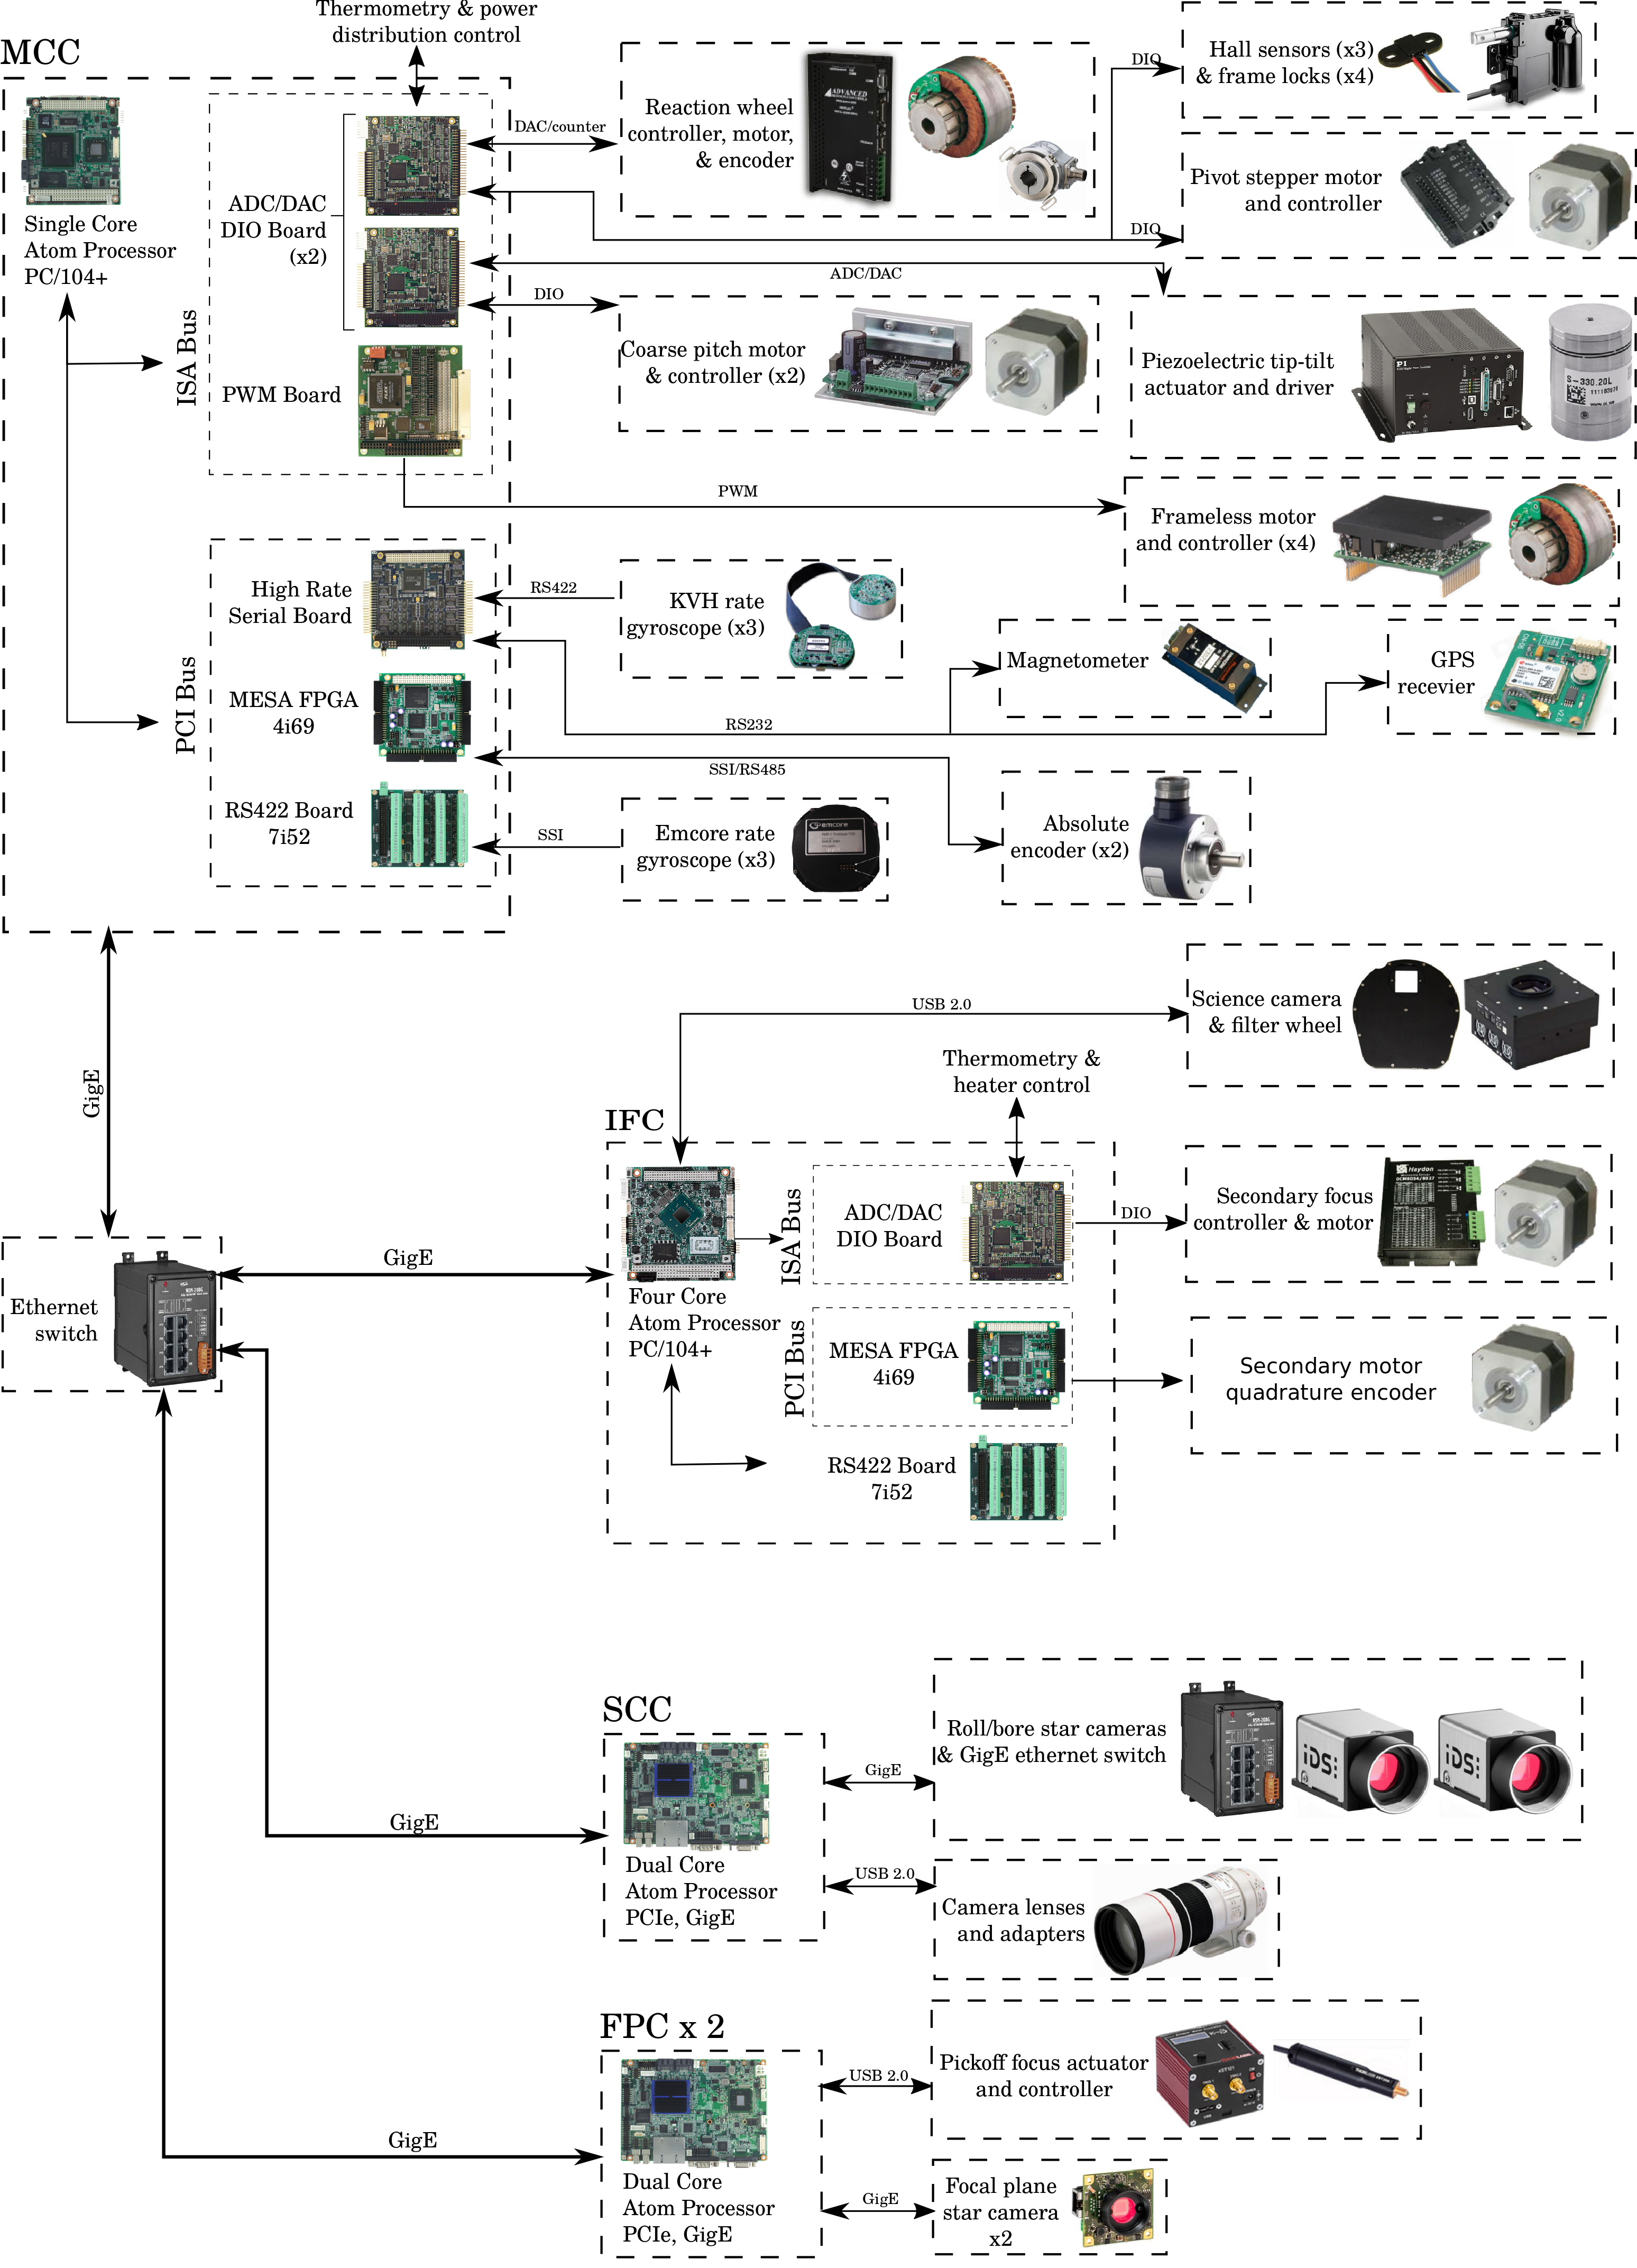
\includegraphics[width=0.95\textwidth]{Hardware/figs/electronics.png}
        \end{center}
        \caption{BIT computer and electronics layout for 2019 flight.}
        \label{fig:electronics}
    \end{small}
\end{figure}

\section{UFO System}
During flight SuperBIT data is nominally transmitted to the ground via satellite communication. Time streams are sent down over each of the
available links (1 MBit LOS, 100 kbps High Gain TDRSS, Iridium) to a central ground computer. Non of the available links are sufficiently fast to transmit SuperBIT's science date during the flight and therefore a hard drive recovery is required.
For a ULDB flight there is a chance that SuperBIT will land in the ocean and thus be unrecoverable. In that scenario the hard drives need to be dropped mid flight separately from the primary payload. The hard drives are parachuted down in a raspberry pi controlled compartment known as the UFO system. This system required the design and building of a power control circuit that enables turning on multiple UFOs on and off separately. The design can be seen in \autoref{fig:UFO circuit}. The implementation was soldering 5 copies of the designed circuit in parallel in order to control 3x UFOs and 1x UFO wifi system. The circuit is a simple latched relay circuit controlled via bit output from the MESA FPGA in the MCC. 

\begin{figure}
    \begin{small}
        \begin{center}
            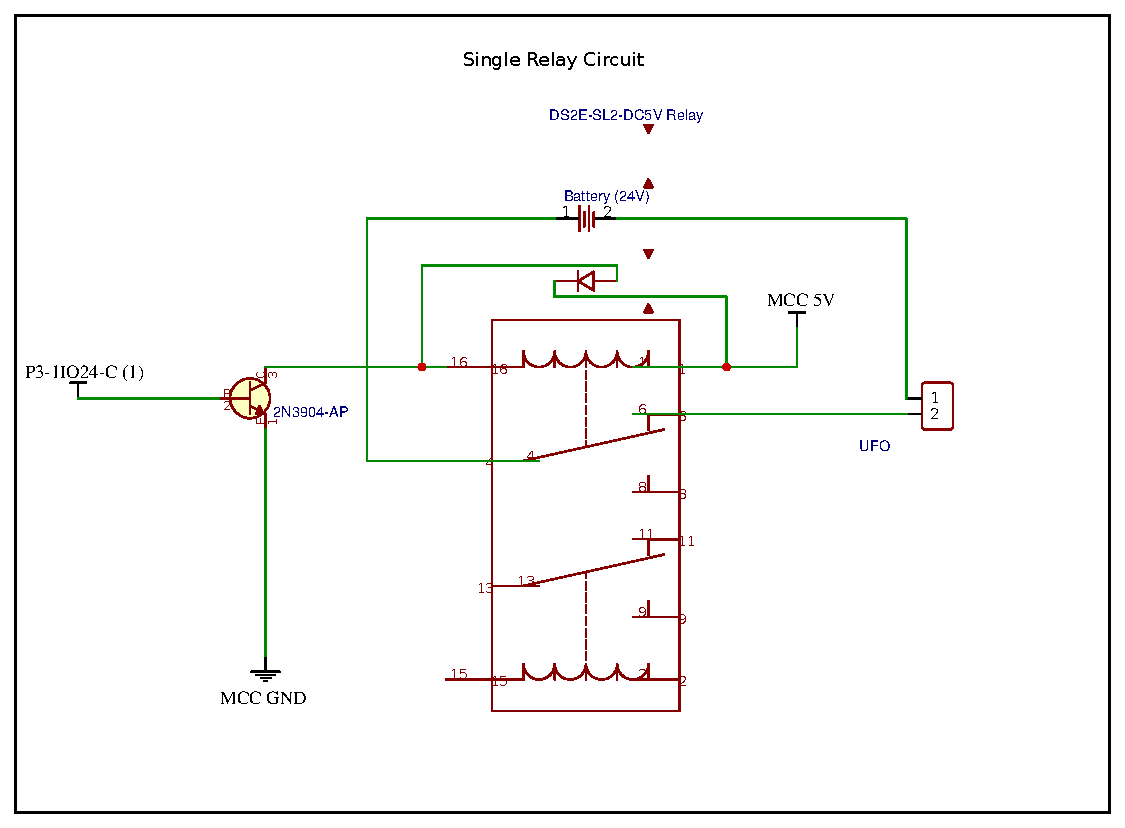
\includegraphics[width=0.95\textwidth]{Hardware/figs/UFO_circ.pdf}
        \end{center}
        \caption{UFO system power control circuit. P3-IO24-C is a sample FPGA output that is fed into a transistor, when the output is pulsed the relay latches on/off turning on the UFO. The UFO is connected directly to SuperBIT's 24V battery system while the relay is isolated and controlled by a 5V power system from the MCC.}
        \label{fig:UFO circuit}
    \end{small}
\end{figure}



\section{Secondary Motors}
The SuperBIT optical system is partially controlled by altering the position of the secondary mirror using three actuators providing tip/tilt/focus motion. The actuators needed to be understood and then have control software written for them. In order to understand the actuators we ran some tests and found the following features. A quadrature encoder is used to feedback position with 8000 encoder ticks per stepper motor revolution. A hall sensor is triggered as a limit switch to enable encoder calibration as well as indicate when the motor has reached min position. After characterizing the behavior of the motors VHDL code was written in order to enable the MESA FPGA in the IFC to interpretate raw encoder data, C wrapper was written to read the fpga write out from the PCI address and have the data available for control feedback.

\section{Baffle Mounting Device}
The star cameras and gyroscopes needed to mount onto the telescope baffle, as a result a mechanism to provide flat mounting surface on the telescope needed to be developed. The primary concern in the design process is to ensure that the mechanism is sufficiently stiff such that no vibrational modes are induced in the telescope and thus increasing the uncertainty in our pointing. We used sorbathane to dampen any vibrations as well as carbon fibre hex to ensure light and stiff material is used. The design can be seen in \autoref{fig:feet}.

\begin{figure}
    \begin{small}
        \begin{center}
            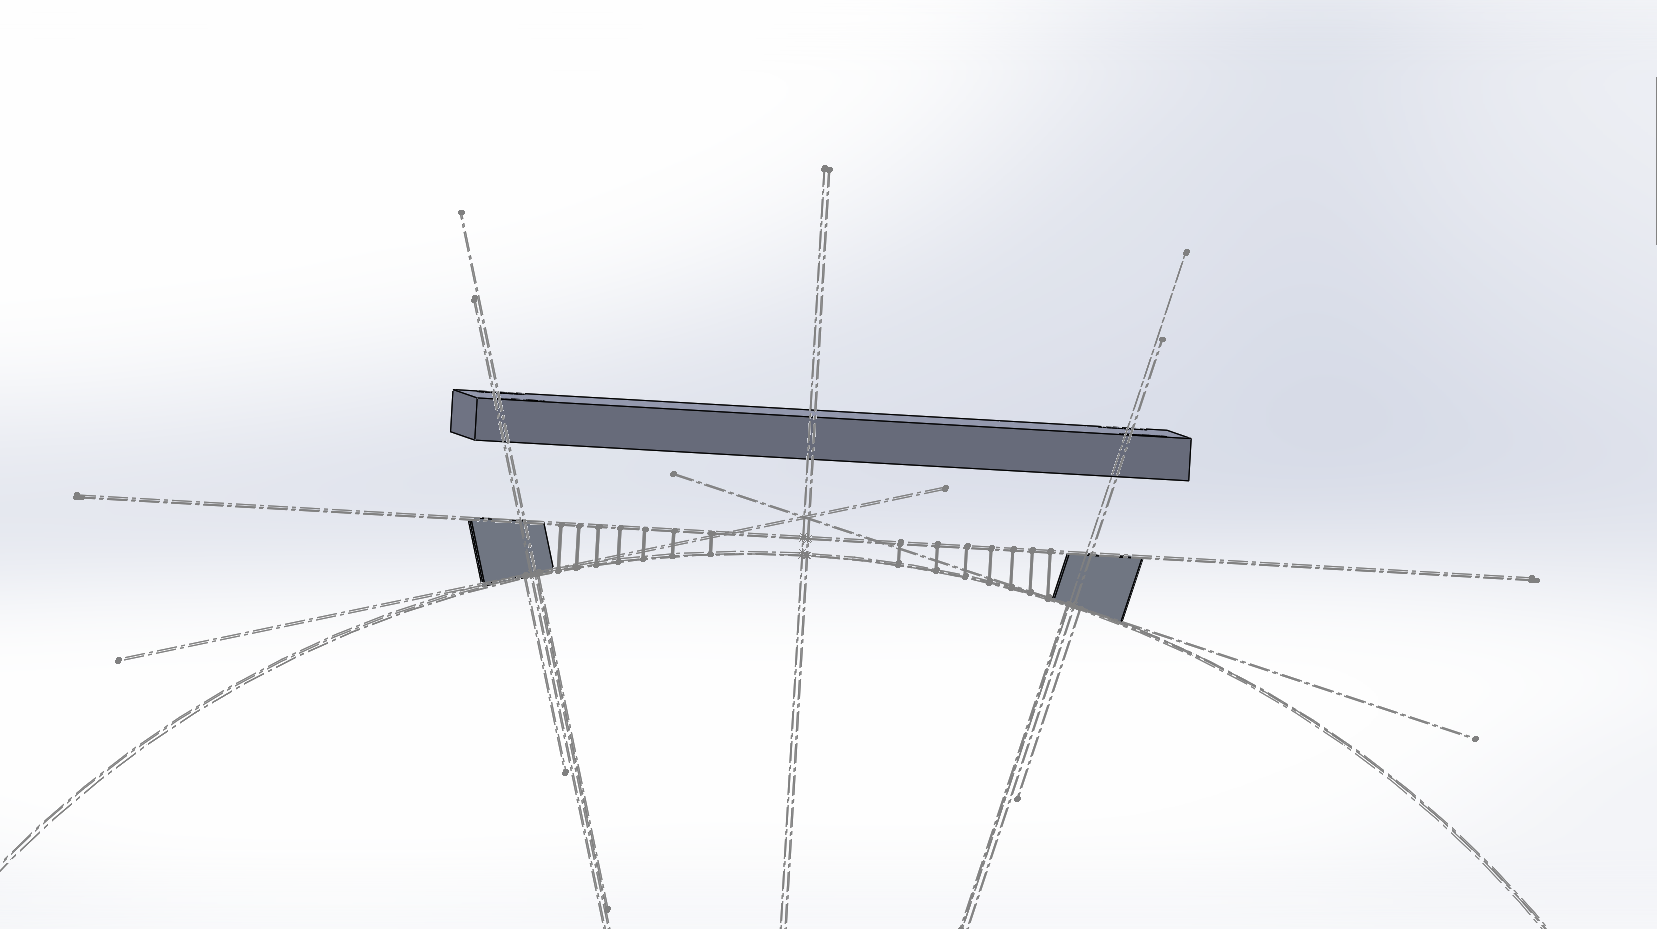
\includegraphics[width=0.95\textwidth]{Hardware/figs/baffle_mount.png}
        \end{center}
        \caption{Baffle mounting system as designed on solidworks. Four angled aluminum feet are mounted directly to the baffle, the feet are angled such that a carbon fibre hex plate can lay flat on all four feet acting as a parallel surface to the telescope baffle's curvature.}
        \label{fig:feet}
    \end{small}
\end{figure}


\section{Battery Boxes}
SuperBIT uses lithium ion batteries that would permanently lose capacity if they drop below a critical temperature and therefore must be thermally controlled. During previous test flights it was empirically found that keeping BIT batteries at the functional temperature used a significant percentage of BIT's total power budget. As a result a new thermal insulation strategy was needed. A brief mathematical analysis was done and found that 2inch thick insolation foam in a heated aluminum box would be sufficient. Some plots for the analysis can be seen at \autoref{fig:boxx mass} \autoref{fig:power loss}. The main considerations where the mass of the insolation box and power insolation. 

\begin{figure}
    \begin{small}
        \begin{center}
            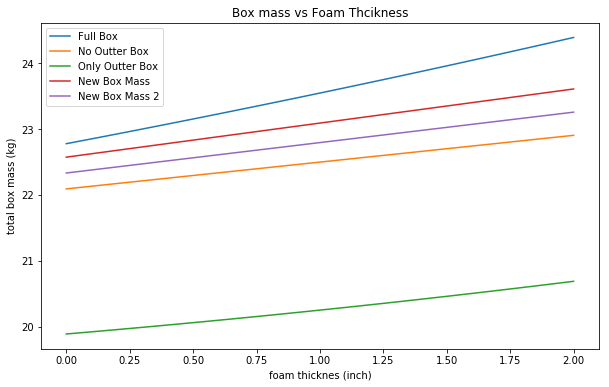
\includegraphics[width=0.95\textwidth]{Hardware/figs/battery_box_mass.png}
        \end{center}
        \caption{The mass of the thermal isolation box as a function of insolation foam thickness}
        \label{fig:boxx mass}
    \end{small}
\end{figure}

\begin{figure}
    \begin{small}
        \begin{center}
            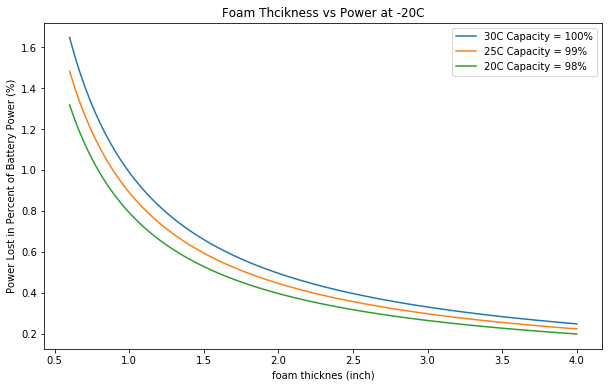
\includegraphics[width=0.95\textwidth]{Hardware/figs/battery_power_loss.png}
        \end{center}
        \caption{Thermal power lost in units of battery power percentage as a function of insolation foam thickness.}
        \label{fig:power loss}
    \end{small}
\end{figure}

\par
Due to the location of the batteries it was found that the new insolation box will require a reduction in the reaction wheel size. A calculation was done to determine the loss in moment of inertia due to the presence of the battery boxes, we found that a total loss of 32\% will be suffered. As a result a new heavier reaction wheel was designed to compensate for the loss. A summary of the analysis is seen in \autoref{fig:rxnwheel}

\begin{figure}
    \begin{small}
        \begin{center}
            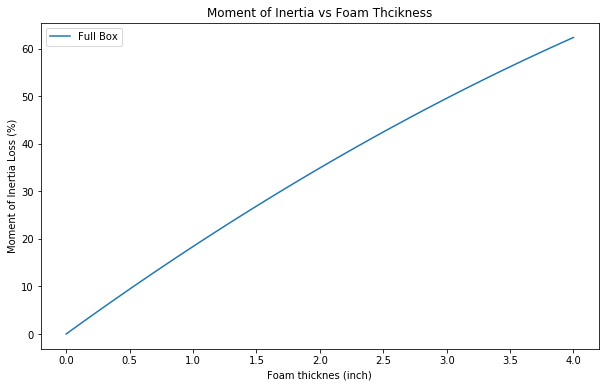
\includegraphics[width=0.95\textwidth]{Hardware/figs/battery_inertia_loss.png}
        \end{center}
        \caption{Loss of moment of inertia of the reaction wheel as a function of insolation foam thickness}
        \label{fig:rxnwheel}
    \end{small}
\end{figure}

\section{Inner Frame Design}
A complete redesign of the BIT electronics layout on the inner frame was completed in order to optimize for space and cable use with respect to the new telescope. This involved the design of new mounting mechanisms for all flight computers and electronics as well as reordering position to optimize for mass balance.


